\documentclass[14pt,a4paper,report]{report}
\usepackage[a4paper, mag=1000, left=2.5cm, right=1cm, top=2cm, bottom=2cm, headsep=0.7cm, footskip=1cm]{geometry}
\usepackage[utf8]{inputenc}
\usepackage[english,russian]{babel}
\usepackage{indentfirst}
\usepackage[dvipsnames]{xcolor}
\usepackage[colorlinks]{hyperref}
\usepackage{listings} 
\usepackage{fancyhdr}
\usepackage{caption}
\usepackage{graphicx}
\hypersetup{
	colorlinks = true,
	linkcolor  = black
}

\usepackage{titlesec}
\titleformat{\chapter}
{\Large\bfseries} % format
{}                % label
{0pt}             % sep
{\huge}           % before-code


\DeclareCaptionFont{white}{\color{white}} 

% Listing description
\usepackage{listings} 
\DeclareCaptionFormat{listing}{\colorbox{gray}{\parbox{\textwidth}{#1#2#3}}}
\captionsetup[lstlisting]{format=listing,labelfont=white,textfont=white}
\lstset{ 
	% Listing settings
	inputencoding = utf8,			
	extendedchars = \true, 
	keepspaces = true, 			  	 % Поддержка кириллицы и пробелов в комментариях
	language = bash,            	 	 % Язык программирования (для подсветки)
	basicstyle = \small\sffamily, 	 % Размер и начертание шрифта для подсветки кода
	numbers = left,               	 % Где поставить нумерацию строк (слева\справа)
	numberstyle = \tiny,          	 % Размер шрифта для номеров строк
	stepnumber = 1,               	 % Размер шага между двумя номерами строк
	numbersep = 5pt,              	 % Как далеко отстоят номера строк от подсвечиваемого кода
	backgroundcolor = \color{white}, % Цвет фона подсветки - используем \usepackage{color}
	showspaces = false,           	 % Показывать или нет пробелы специальными отступами
	showstringspaces = false,    	 % Показывать или нет пробелы в строках
	showtabs = false,           	 % Показывать или нет табуляцию в строках
	frame = single,              	 % Рисовать рамку вокруг кода
	tabsize = 2,                  	 % Размер табуляции по умолчанию равен 2 пробелам
	captionpos = t,             	 % Позиция заголовка вверху [t] или внизу [b] 
	breaklines = true,           	 % Автоматически переносить строки (да\нет)
	breakatwhitespace = false,   	 % Переносить строки только если есть пробел
	escapeinside = {\%*}{*)}      	 % Если нужно добавить комментарии в коде
}

\begin{document}

\def\contentsname{Contents}

% Titlepage
\begin{titlepage}
	\begin{center}
		\textsc{Peter the Great St.Petersburg Polytechnic University\\[5mm]
			Department of Computer Systems \& Software Engineering}
		
		\vfill
		
		\textbf{Laboratory report №6\\[3mm]
			Discipline: «Information Security»\\[3mm]
			Theme: «OWASP WebGoat»\\[41mm]
		}
	\end{center}
	
	\hfill
	\begin{minipage}{.4\textwidth}
		Made by student:\\[2mm] 
		Volkova M.D.\\
		Group: 13541/2\\[5mm]
		
		Lecturer:\\[2mm] 
		Bogach N.V.
	\end{minipage}
	\vfill
	\begin{center}
		Saint-Petersburg\\ \the\year\ y.
	\end{center}
\end{titlepage}

% Contents
\tableofcontents
\clearpage

\chapter{Laboratory work №6}

\section{Work purpose}

WebGoat is a deliberately insecure web application maintained by OWASP designed to teach web application security.

\section{Task}

\subsubsection{Study}

\begin{enumerate}
	\item Using OWASP Top Ten Project study top 10 web vulnerabilities.
\end{enumerate}

\subsubsection{Exercises}

\begin{enumerate}
	\item Install and launch WebGoat
	\item Launch ZAP security scanner, configure it as a local proxy-server. NOTE: Please, use different port numbers for ZAP and WebGoat.
	\item Launch Mantra, set it to use ZAP as proxy-server (Top left -> Tools -> Settings)
	\item Follow WebGoat LESSONS
\end{enumerate}

\section{Study}

\subsection{Using OWASP Top Ten Project study top 10 web vulnerabilities}

\begin{enumerate}
	\item \textbf{Injection Injection} flaws, such as SQL, OS, XXE, and LDAP injection occur when untrusted
	data is sent to an interpreter as part of a command or query. The attacker’s hostile data
	can trick the interpreter into executing unintended commands or accessing data without
	proper authorization.
	\item \textbf{Broken Authentication and Session Management} Application functions related to authentication
	and session management are often implemented incorrectly, allowing attackers
	to compromise passwords, keys, or session tokens, or to exploit other implementation
	flaws to assume other users’ identities (temporarily or permanently).
	\item \textbf{Cross-Site Scripting (XSS)} XSS flaws occur whenever an application includes untrusted
	data in a new web page without proper validation or escaping, or updates an existing
	web page with user supplied data using a browser API that can create JavaScript. XSS
	allows attackers to execute scripts in the victim’s browser which can hijack user sessions,
	deface web sites, or redirect the user to malicious sites.
	\item \textbf{Insecure Direct Object References} Restrictions on what authenticated users are allowed
	to do are not properly enforced. Attackers can exploit these flaws to access unauthorized
	functionality and/or data, such as access other users’ accounts, view sensitive files,
	modify other users’ data, change access rights, etc.
	\item \textbf{Security Misconfiguration} Good security requires having a secure configuration defined
	and deployed for the application, frameworks, application server, web server, database
	server, platform, etc. Secure settings should be defined, implemented, and maintained,
	as defaults are often insecure. Additionally, software should be kept up to date.
	\item \textbf{Sensitive Data Exposure} Many web applications and APIs do not properly protect sensitive
	data, such as financial, healthcare, and PII. Attackers may steal or modify such
	weakly protected data to conduct credit card fraud, identity theft, or other crimes. Sensitive
	data deserves extra protection such as encryption at rest or in transit, as well as
	special precautions when exchanged with the browser.
	\item \textbf{Missing Function Level Access Control} The majority of applications and APIs lack the
	basic ability to detect, prevent, and respond to both manual and automated attacks. Attack
	protection goes far beyond basic input validation and involves automatically detecting,
	logging, responding, and even blocking exploit attempts. Application owners also
	need to be able to deploy patches quickly to protect against attacks.
	\item\textbf{ Cross-Site Request Forgery (CSRF)} A CSRF attack forces a logged-on victim’s browser
	to send a forged HTTP request, including the victim’s session cookie and any other automatically
	included authentication information, to a vulnerable web application. Such an
	attack allows the attacker to force a victim’s browser to generate requests the vulnerable
	application thinks are legitimate requests from the victim.
	\item\textbf{ Using Components with Known Vulnerabilities} Components, such as libraries, frameworks,
	and other software modules, run with the same privileges as the application.
	If a vulnerable component is exploited, such an attack can facilitate serious data loss
	or server takeover. Applications and APIs using components with known vulnerabilities
	may undermine application defenses and enable various attacks and impacts.
	\item \textbf{Unvalidated Redirects and Forwards} Modern applications often involve rich client applications
	and APIs, such as JavaScript in the browser and mobile apps, that connect
	to an API of some kind (SOAP/XML, REST/JSON, RPC, GWT, etc.). These APIs are often
	unprotected and contain numerous vulnerabilities.
\end{enumerate}

\section{Exercises}

\subsection{Install and launch WebGoat}

Download OWASP webgoat version 7.1 from the official website of the company. Then run it by the following command:

\lstinputlisting{listings/1.log}

Now the server is available at http://localhost:65100 address:

\begin{figure}[h!]
	\centering
	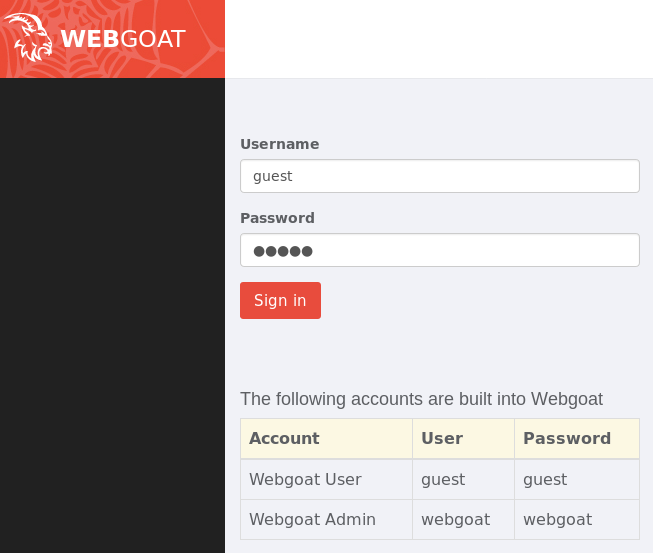
\includegraphics[scale = 0.65]{images/1.png}
	\caption{Webgoat login page}
\end{figure}

After that, a redirect to the main page of the site:

\begin{figure}[h!]
	\centering
	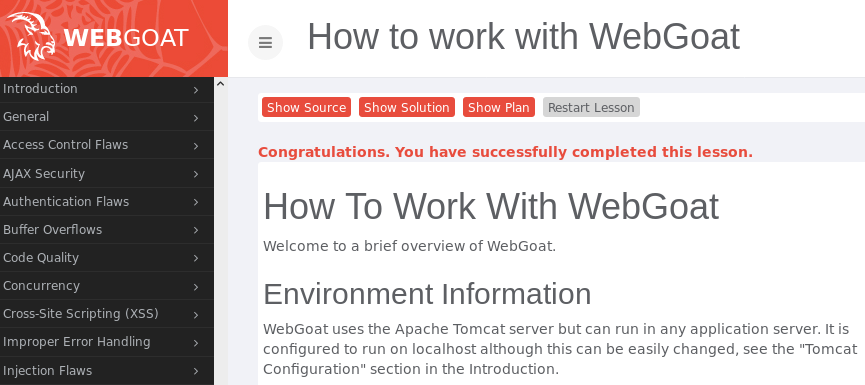
\includegraphics[scale = 0.65]{images/2.png}
	\caption{Webgoat start page}
\end{figure}

\subsection{Launch ZAP security scanner, configure it as a local proxy-server}

Download OWASP ZAP security scanner from the official website of the company. Then run it by the following command:

\lstinputlisting{listings/2.log}

After that, the application starts:

\begin{figure}[h!]
	\centering
	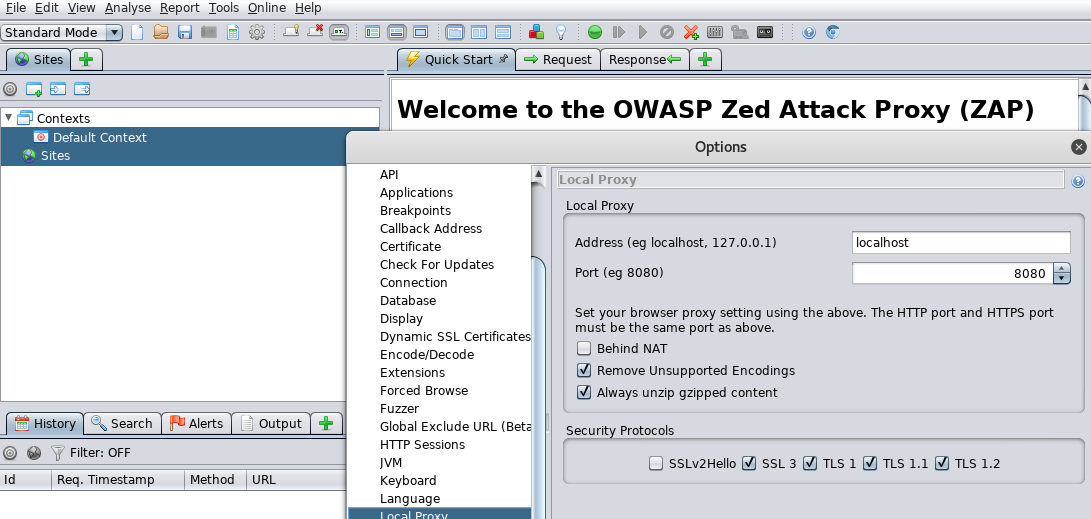
\includegraphics[scale = 0.60]{images/3.png}
	\caption{ZAP start window and port configuring}
\end{figure}

\clearpage

Let's configure firefox proxy server:

\begin{figure}[h!]
	\centering
	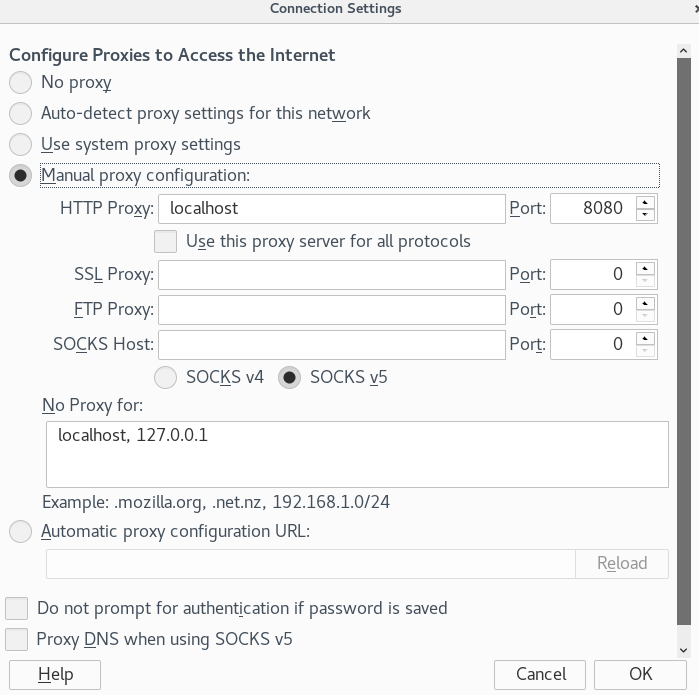
\includegraphics[scale = 0.60]{images/4.png}
	\caption{Firefox proxy server configuration}
\end{figure}

After configuring the proxy server, the ZAP scanner displays traffic information:

\begin{figure}[h!]
	\centering
	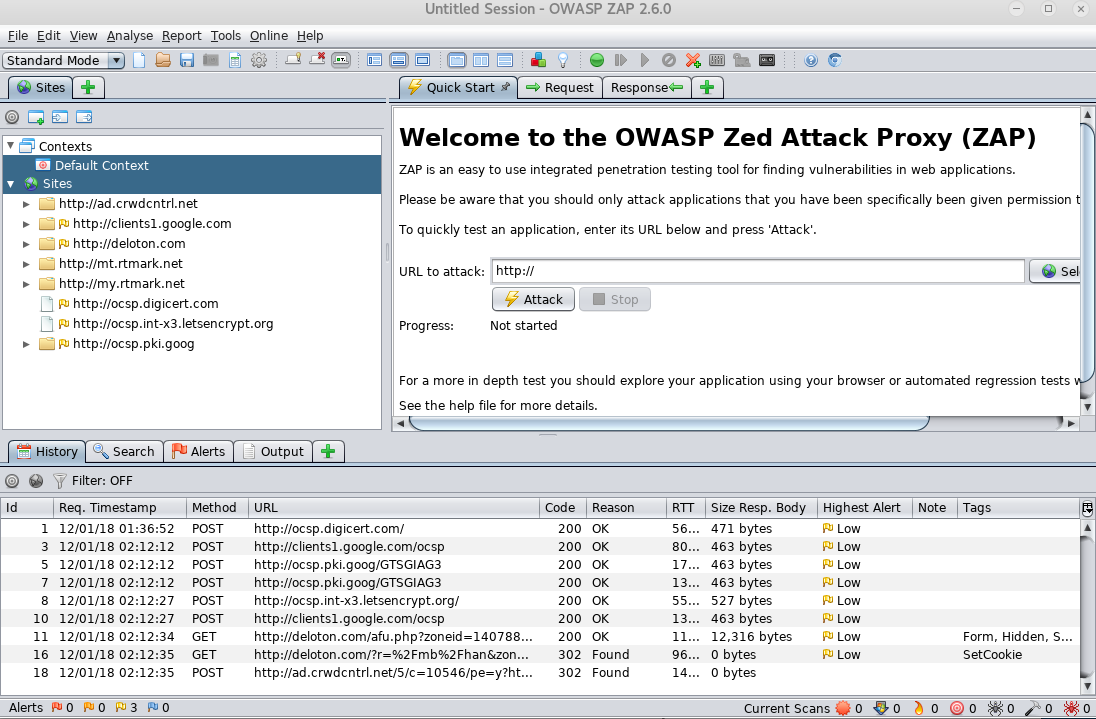
\includegraphics[scale = 0.50]{images/5.png}
	\caption{Traffic information}
\end{figure}

\subsection{Vulnerabilities using}

\subsubsection{SQL Injection}

When selecting a weather station, the station field value changes: the Columbia field has a value of 101. 

\begin{figure}[h!]
	\centering
	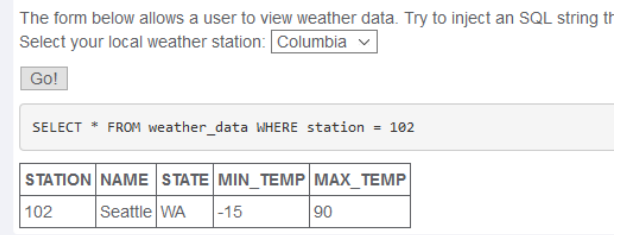
\includegraphics[scale = 0.61]{images/6.png}
	\caption{Standart SQL result}
\end{figure}

Let's change the type of the html element to <input type = "text"> and set the injection value to "101 or 1 = 1" to display all table values:

\begin{figure}[h!]
	\centering
	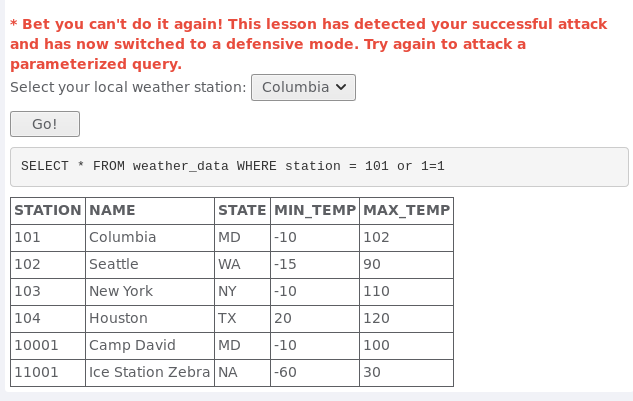
\includegraphics[scale = 0.61]{images/7.png}
	\caption{SQL result after an injection}
\end{figure}

\subsubsection{Broken Authentication and Session Management}

With the help of the site https://howsecureismypassword.net/ it is necessary to enter the time for hacking each of the passwords:

\begin{figure}[h!]
	\centering
	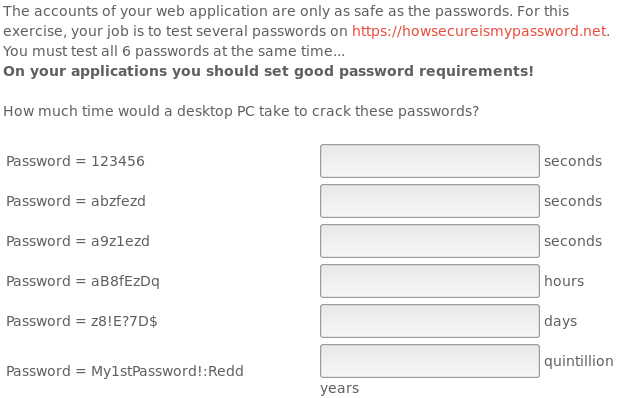
\includegraphics[scale = 0.60]{images/8.png}
	\caption{password strength}
\end{figure}

Results:

\begin{figure}[h!]
	\centering
	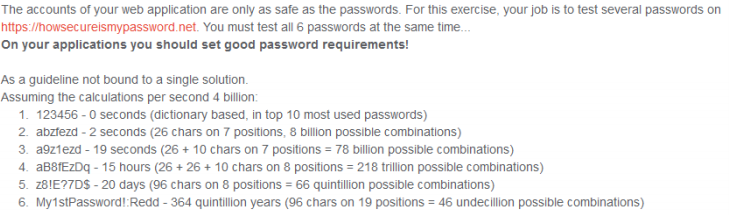
\includegraphics[scale = 0.60]{images/9.png}
	\caption{Password strength results}
\end{figure}

\subsubsection{Cross-Site Scripting (XSS)}

In this task need to catch user login and passwrod, using XSS and HTML insertion: 

\begin{figure}[h!]
	\centering
	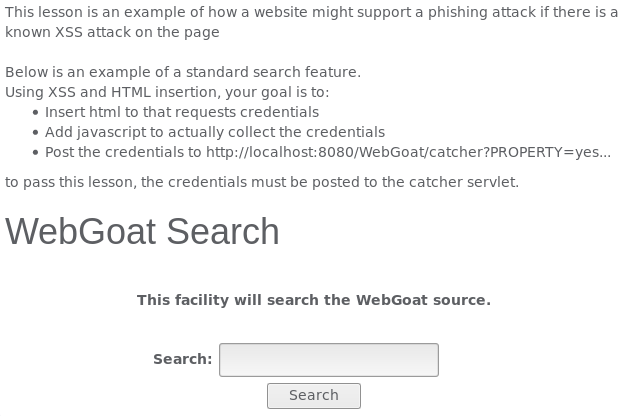
\includegraphics[scale = 0.71]{images/10.png}
	\caption{}
\end{figure}

To complete this task put the following code into "search" field:

\lstinputlisting{listings/3.log}

As a result, a window with the user's login and password is displayed:

\begin{figure}[h!]
	\centering
	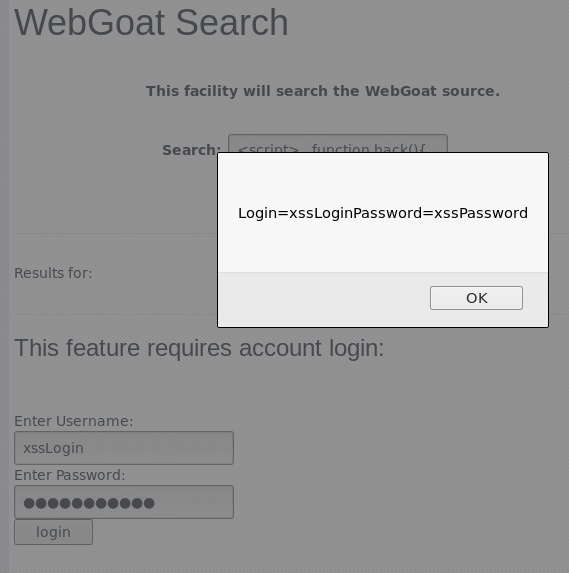
\includegraphics[scale = 0.50]{images/11.png}
	\caption{Result of the XSS hack}
\end{figure}

\subsubsection{Insecure Direct Object References}

The next task is to get the password that is sent via HTTP protocol:

\begin{figure}[h!]
	\centering
	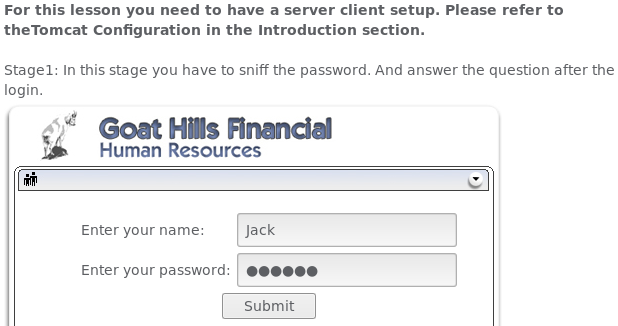
\includegraphics[scale = 0.50]{images/12.png}
	\caption{Simple form to hack}
\end{figure}

This form uses the HTTP protocol. The password can be easily stolen with a simple traffic analysis. With the help of Wireshark a password was received -- sniffy:

\begin{figure}[h!]
	\centering
	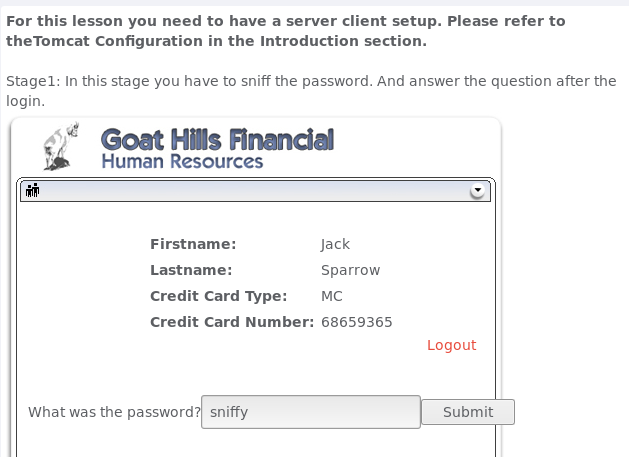
\includegraphics[scale = 0.50]{images/13.png}
	\caption{The result of the task}
\end{figure}

\section{Conclusion}

In this paper, OWASP WebGoat was studied. This program was created to teach developers to protect against the main vulnerabilities of the web server. Such lessons can be useful not only for beginners, but also for experienced developers.





\end{document}